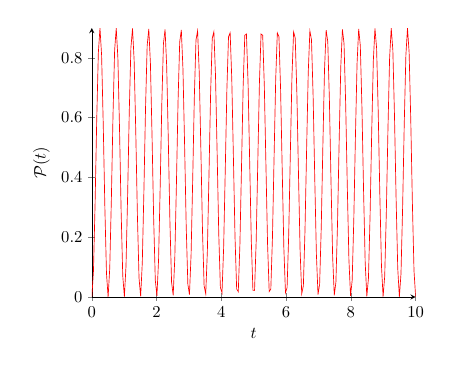
\begin{tikzpicture}[scale=0.6]
\shothandoff{:!}
  \begin{axis}[
    axis lines = left,
    xlabel = \(t\),
    ylabel = {\(\mathcal{P}(t)\)},
]
\addplot [
    domain=0:10, 
    samples=200, 
    color=red,
]
{9/10*sin(deg(2*pi*x))*sin(deg(2*pi*x))};

\end{axis}

\shothandon{:!}
\end{tikzpicture}